\documentclass{beamer}
\usetheme{metropolis}
\usepackage{graphicx}
\usepackage{diagbox}
\usepackage{tcolorbox}
\title{Computer Logic and Digital Circuit Design (PHYS306/COSC330): Unit 3}
\author{Jordan Hanson}
\institute{Whittier College Department of Physics and Astronomy}

\begin{document}
\maketitle

\section{Summary}

\begin{frame}{Unit 3 Summary}
\alert{Reading: chapter 7} \\
We now know how to generate and process digital data. We can do algebra, compare numbers, encode, decode, and multiplex.  \textit{How does memory work?  How is information held in digital systems?}
\begin{enumerate}
\item S-R latches
\begin{itemize}
\item Basic latch, de-bounce
\item Gated latch
\item D-latch
\end{itemize}
\item Flip-flops
\begin{itemize}
\item JK flip-flops
\item Synchronous vs. level-sensitive
\end{itemize}
\end{enumerate}
\end{frame}

\section{S-R Latches}

\begin{frame}{S-R Latches}
\begin{figure}
\centering
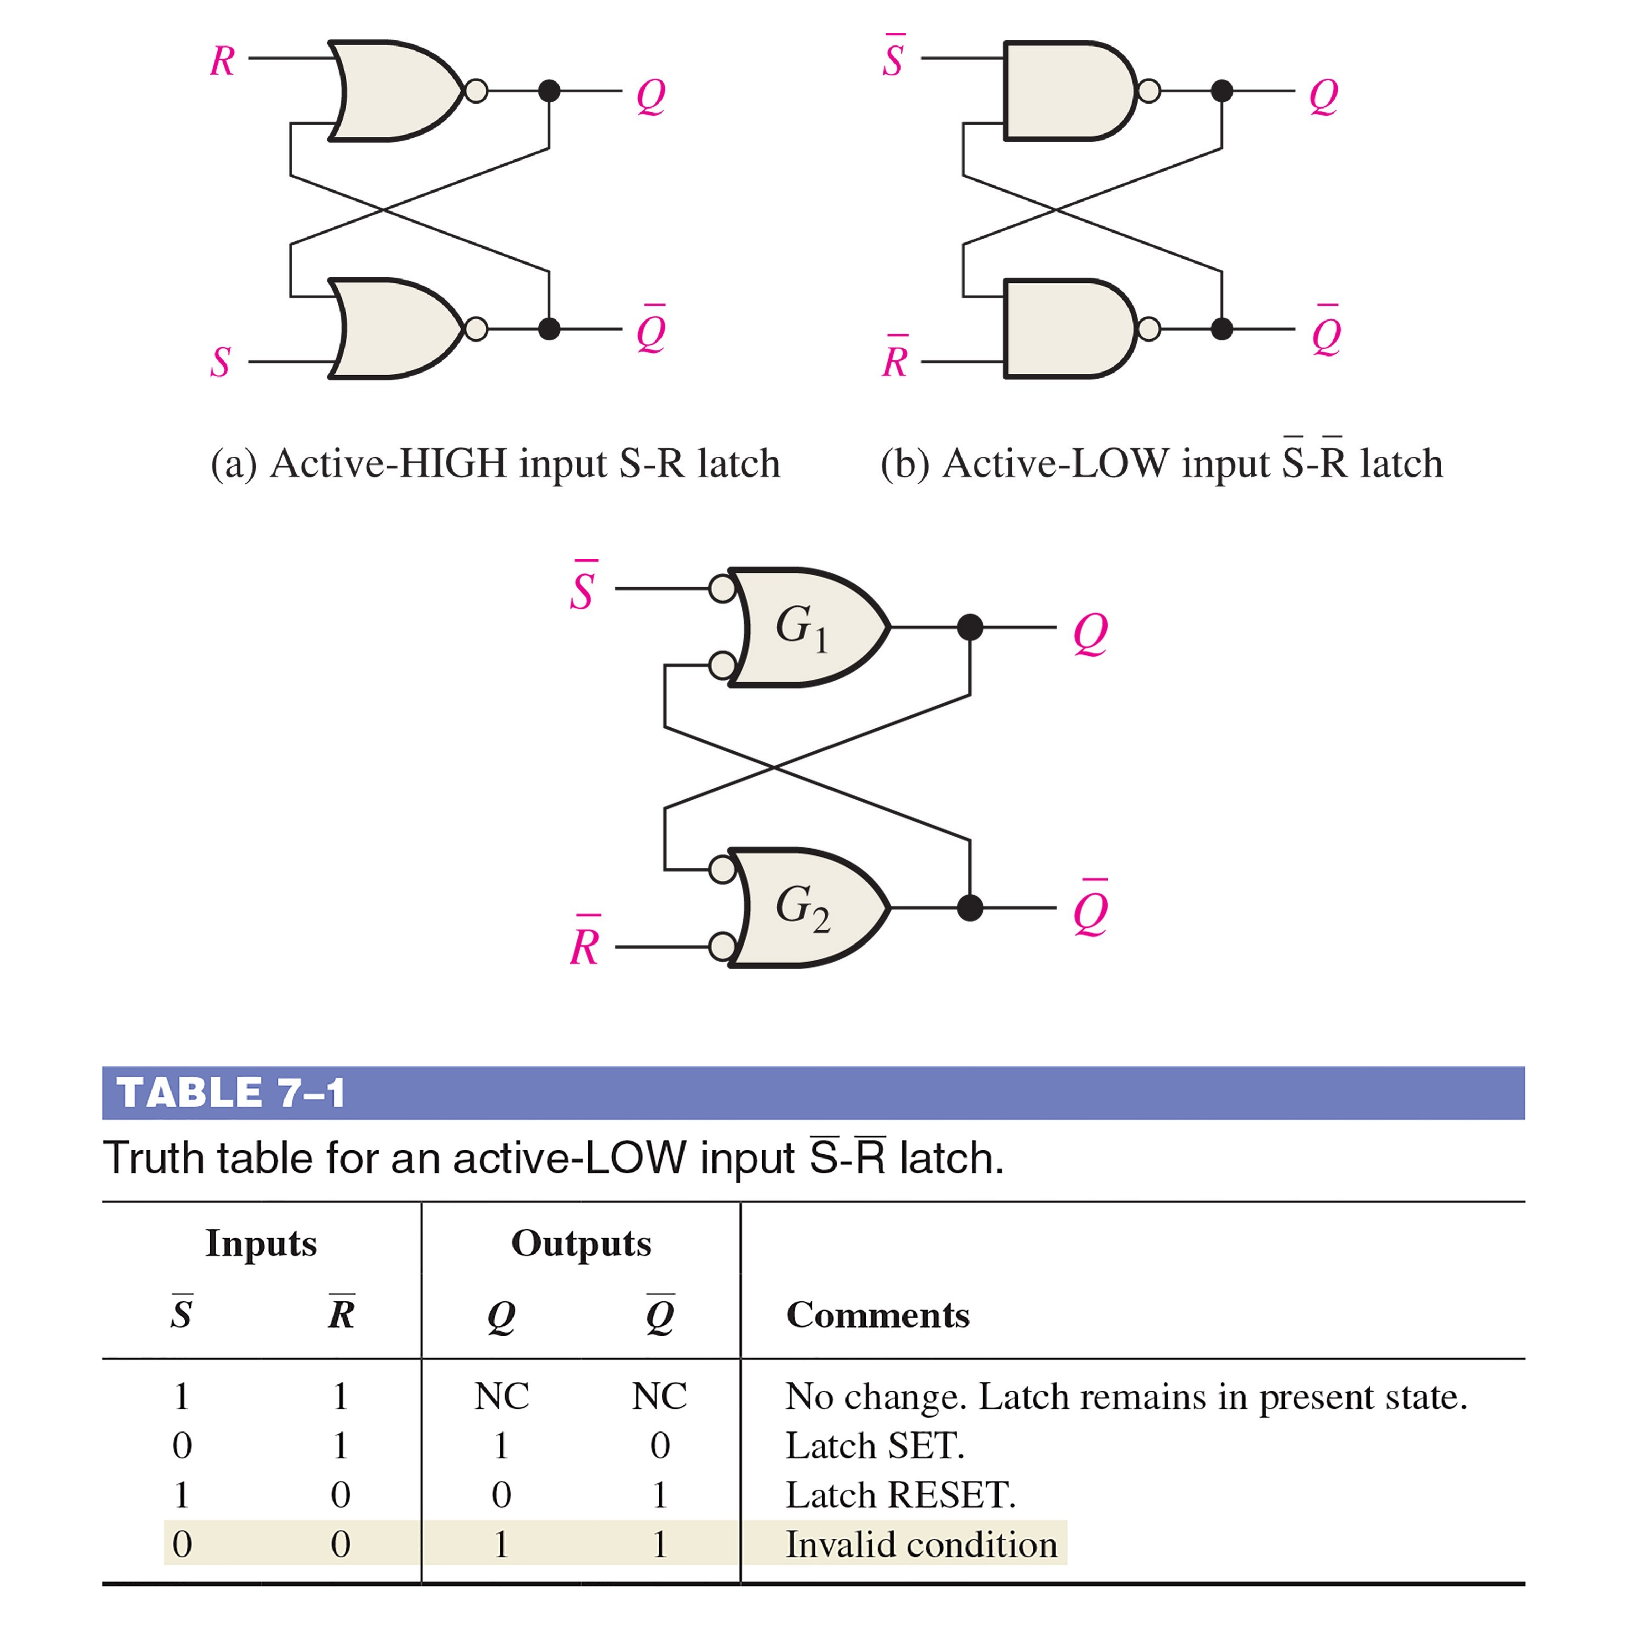
\includegraphics[width=0.55\textwidth]{figures/SR1.pdf}
\caption{\label{fig:sr1} An S-R latch is a \textit{multivibrator} that holds its state when SET, or RESET.}
\end{figure}
\end{frame}

\begin{frame}{S-R Latches}
\begin{figure}
\centering
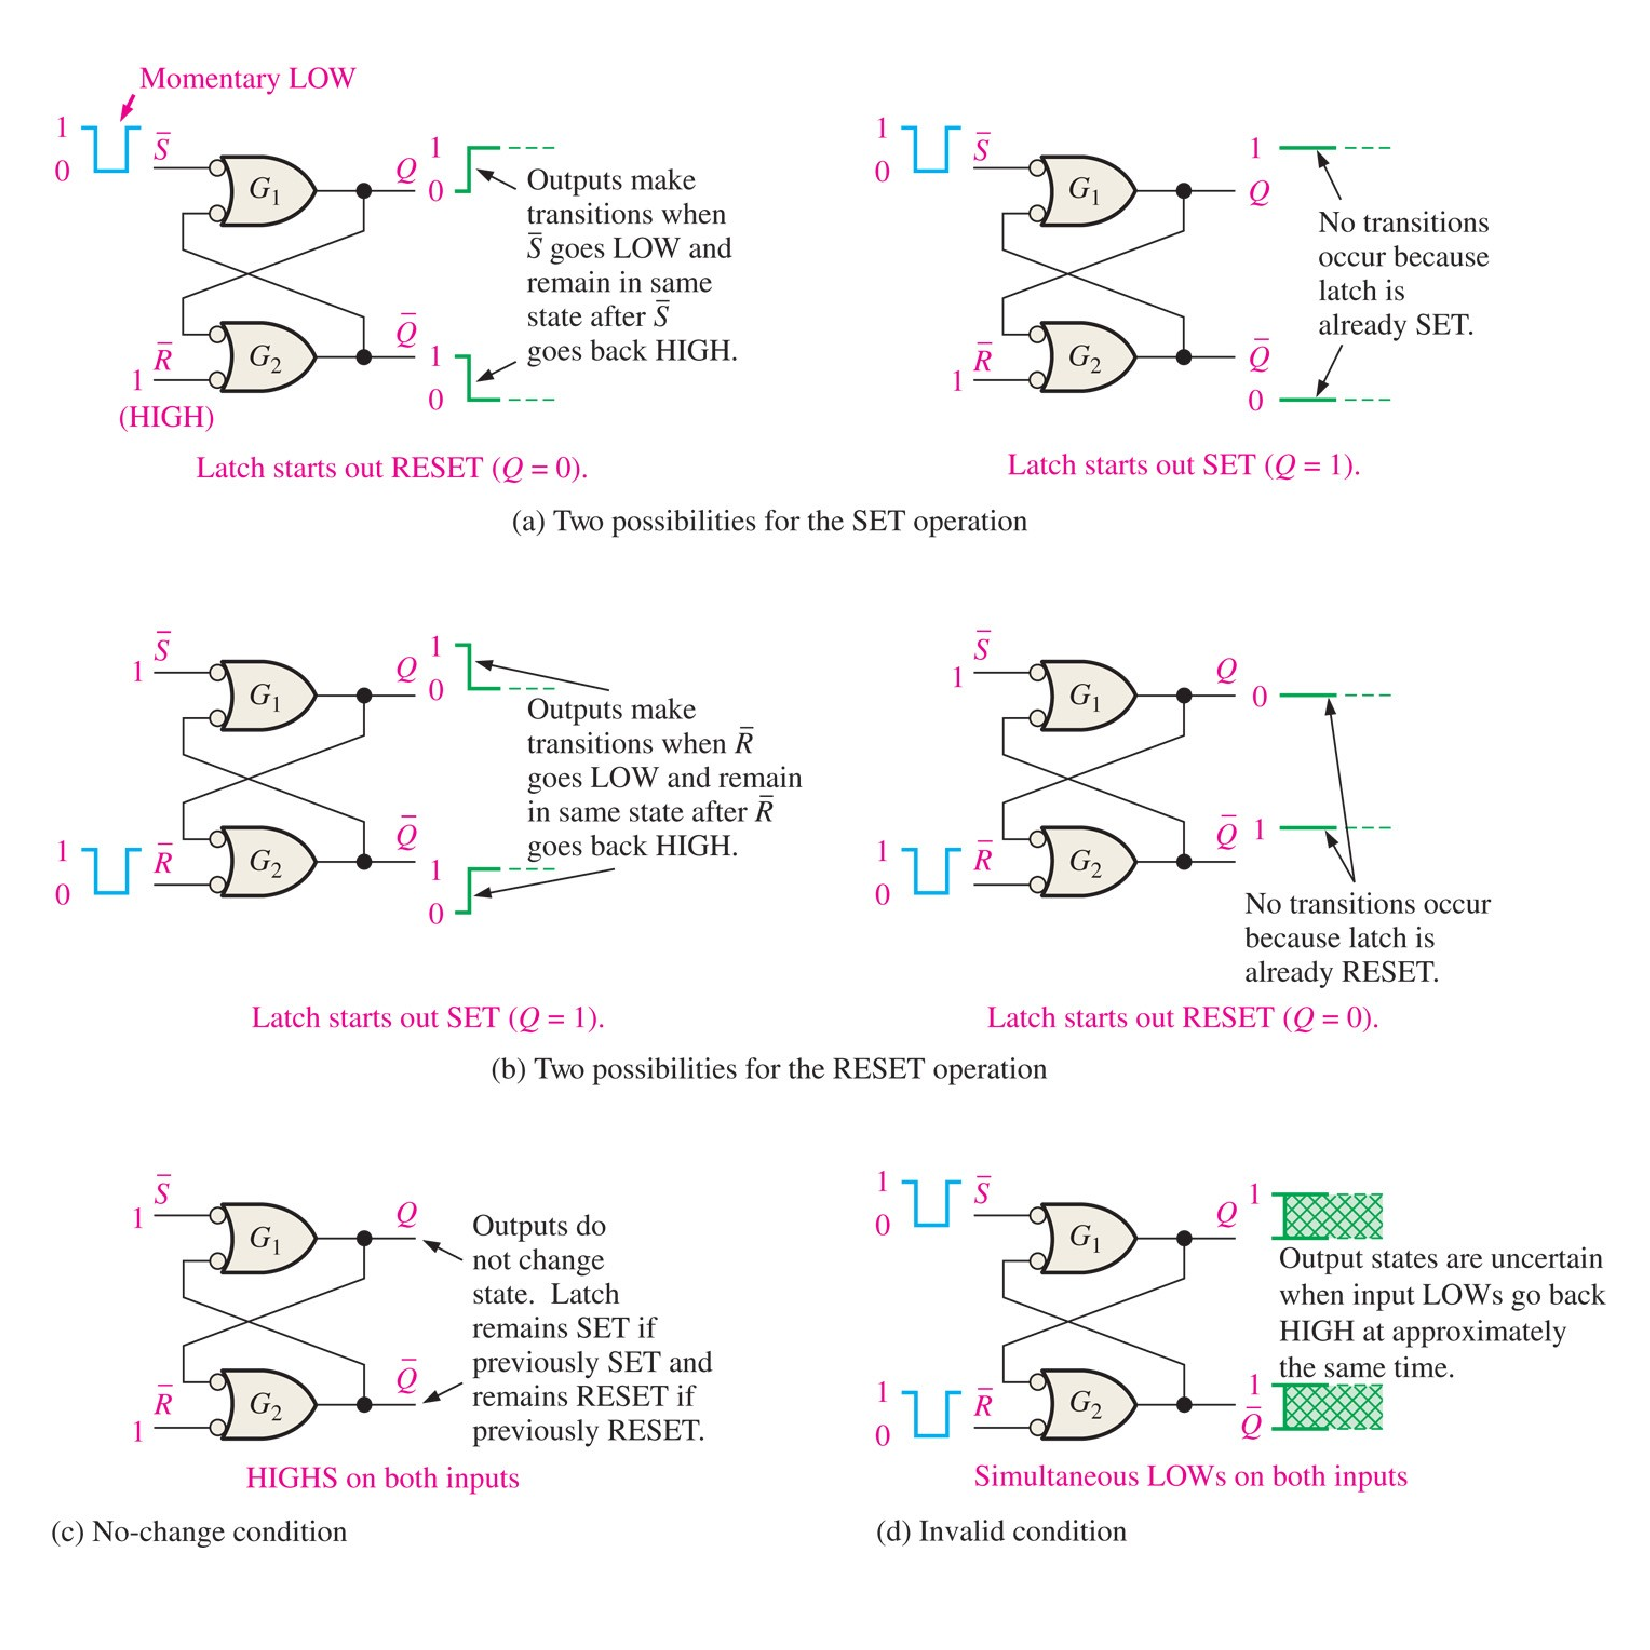
\includegraphics[width=0.55\textwidth]{figures/SR2.pdf}
\caption{\label{fig:sr2} Summary of potential states of a basic S-R latch.}
\end{figure}
\end{frame}

\begin{frame}{S-R Latches}
\begin{figure}
\centering
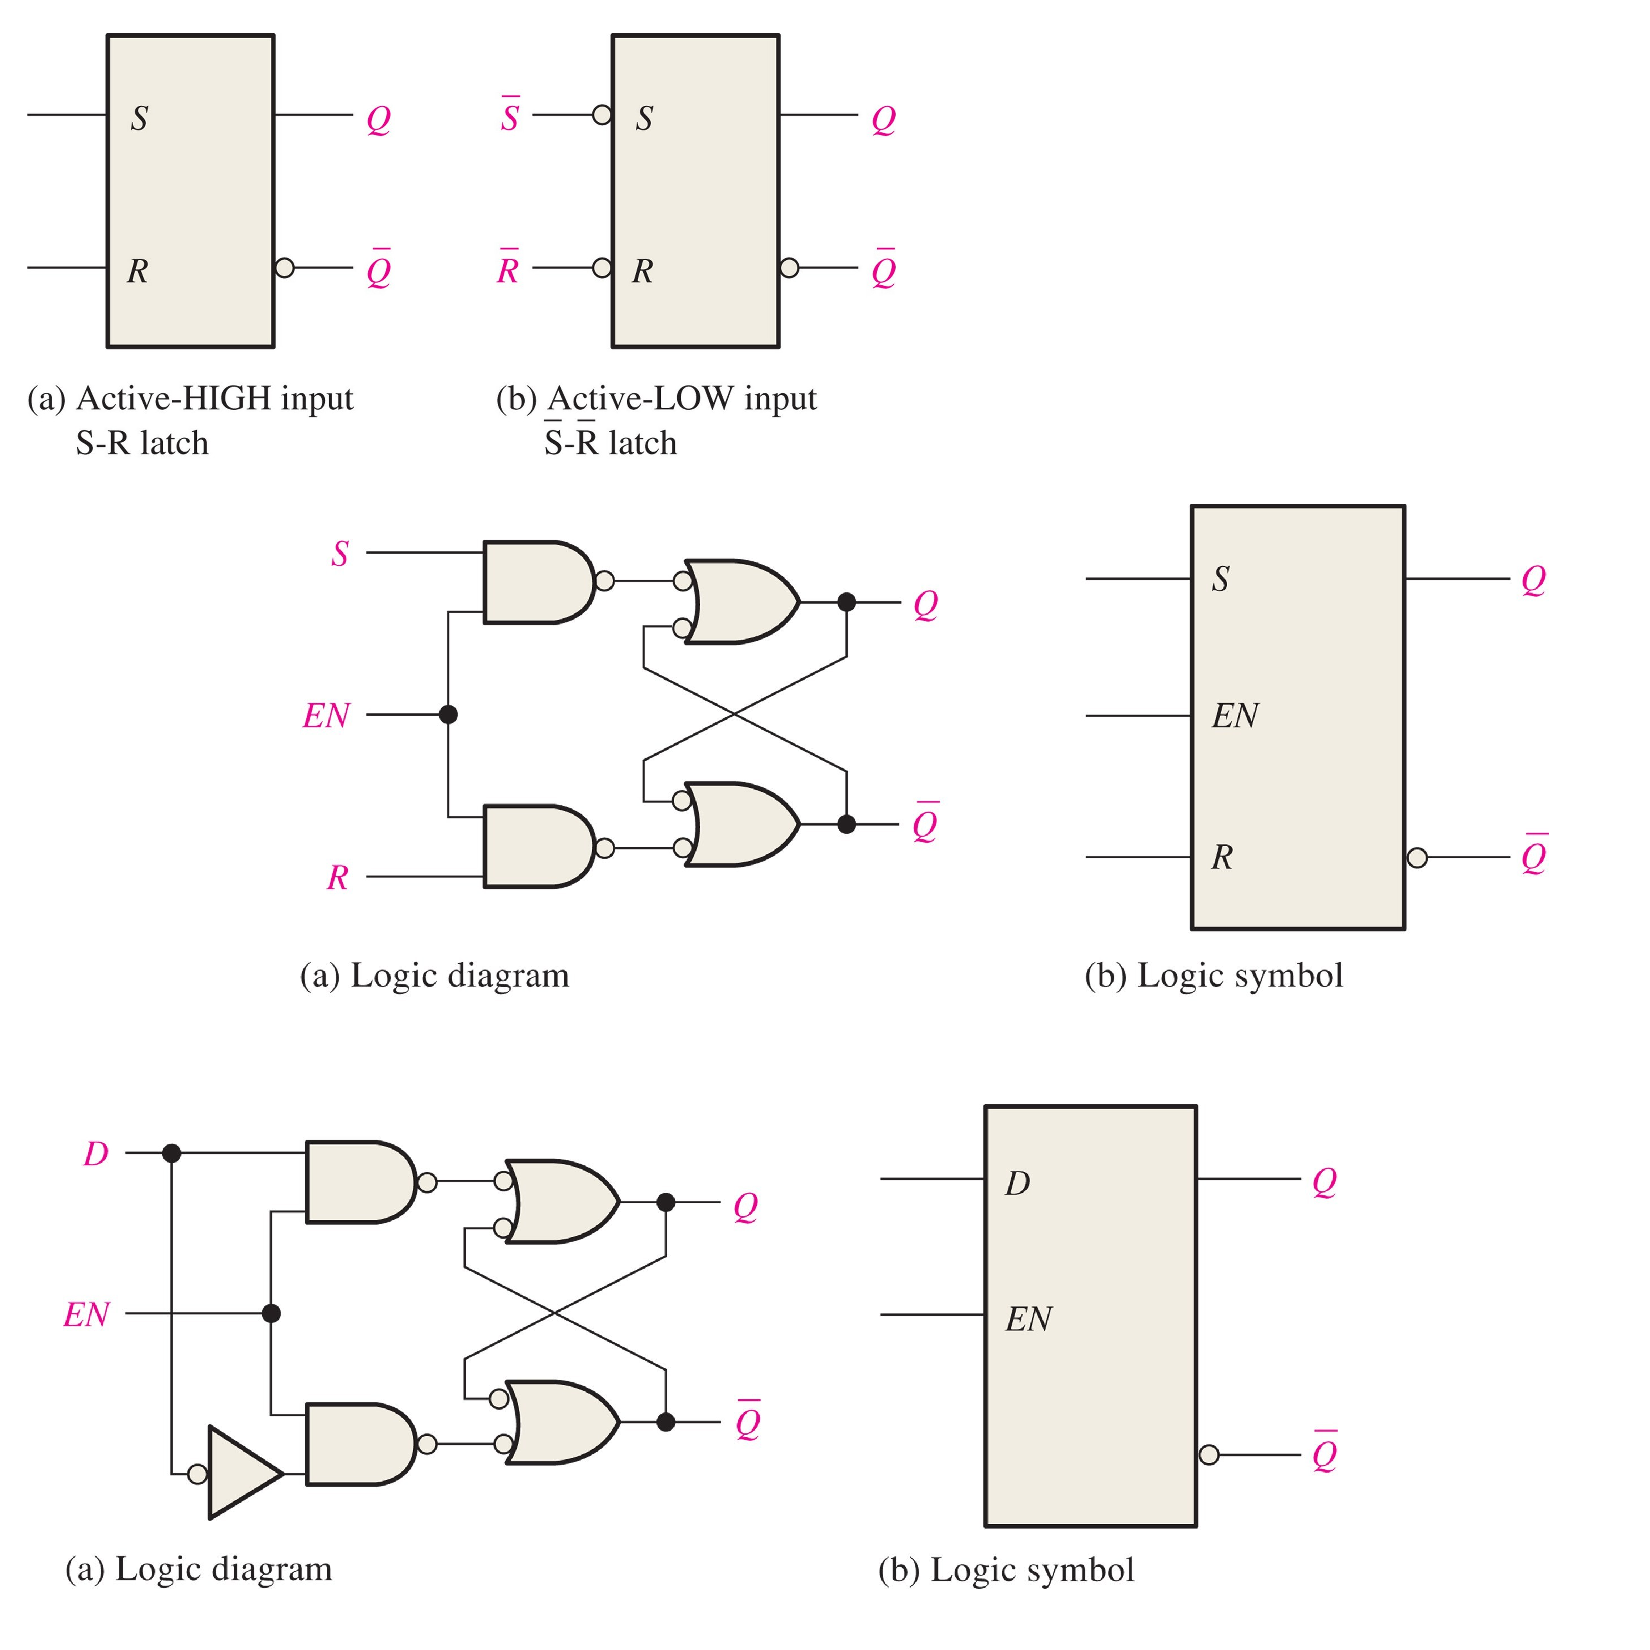
\includegraphics[width=0.55\textwidth]{figures/SR3.pdf}
\caption{\label{fig:sr3} The basic, gate-enabled, and D-latch systems.  For the latter two, both the gate and symbol are shown.}
\end{figure}
\end{frame}

\begin{frame}{S-R Latches}
\begin{figure}
\centering
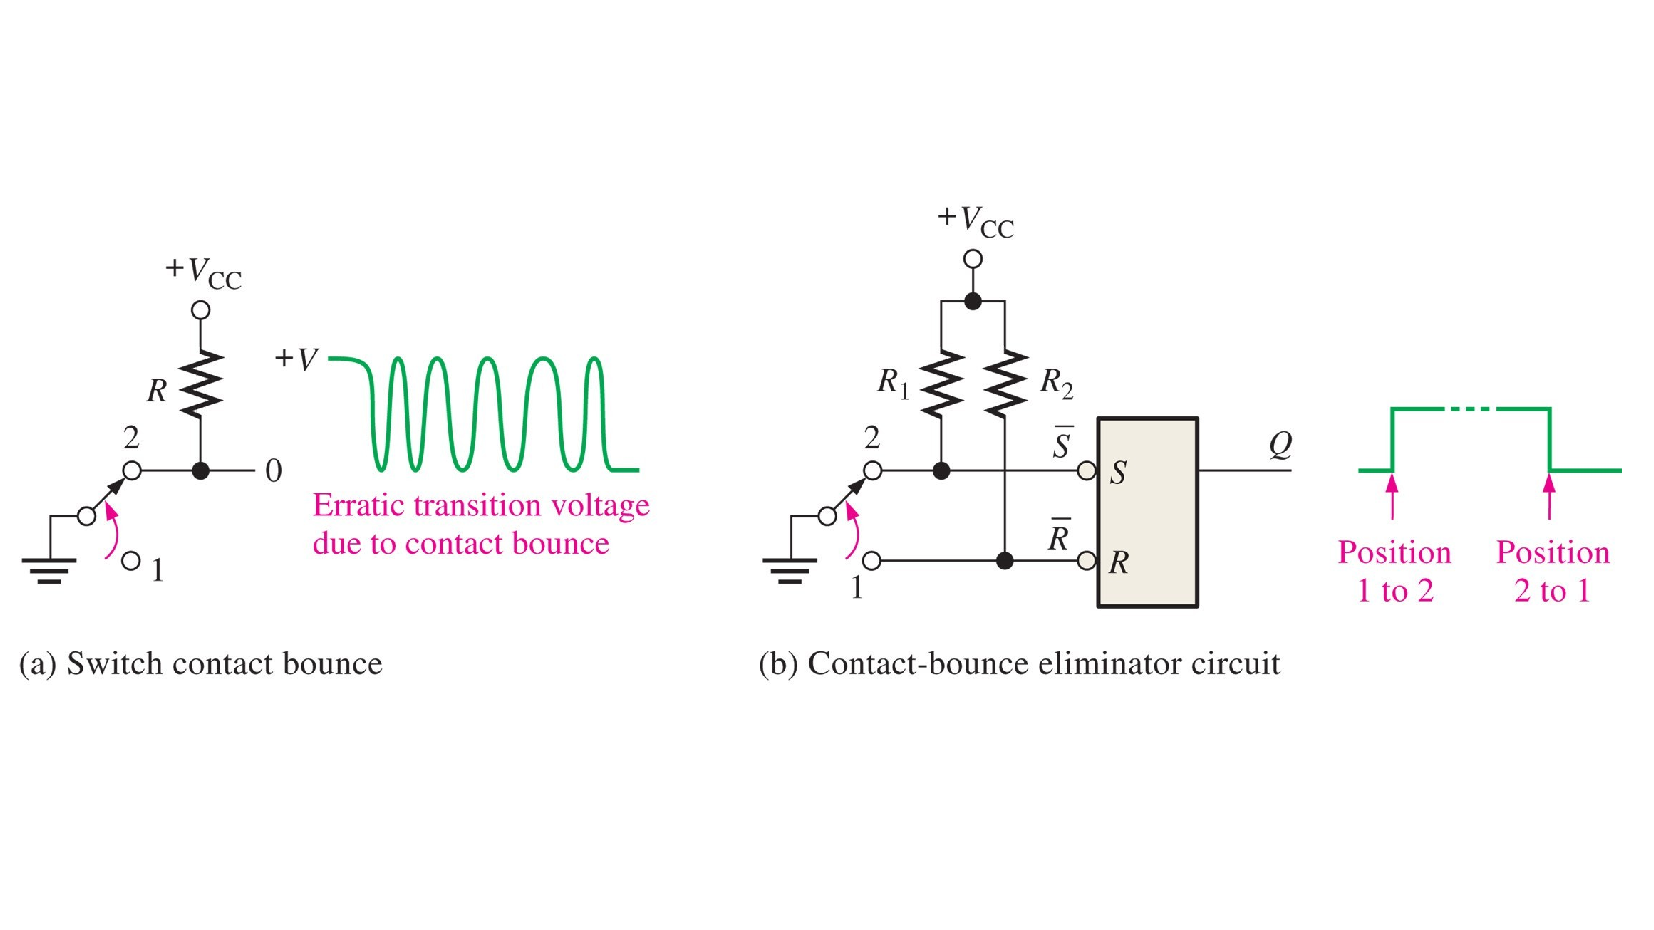
\includegraphics[width=0.85\textwidth]{figures/SR4.pdf}
\caption{\label{fig:sr4} De-bouncing is important any time a mechanical switch is meant to interact with digital logic.}
\end{figure}
\end{frame}

\section{Flip Flops}

\begin{frame}{Flip-Flops}
\begin{figure}
\centering
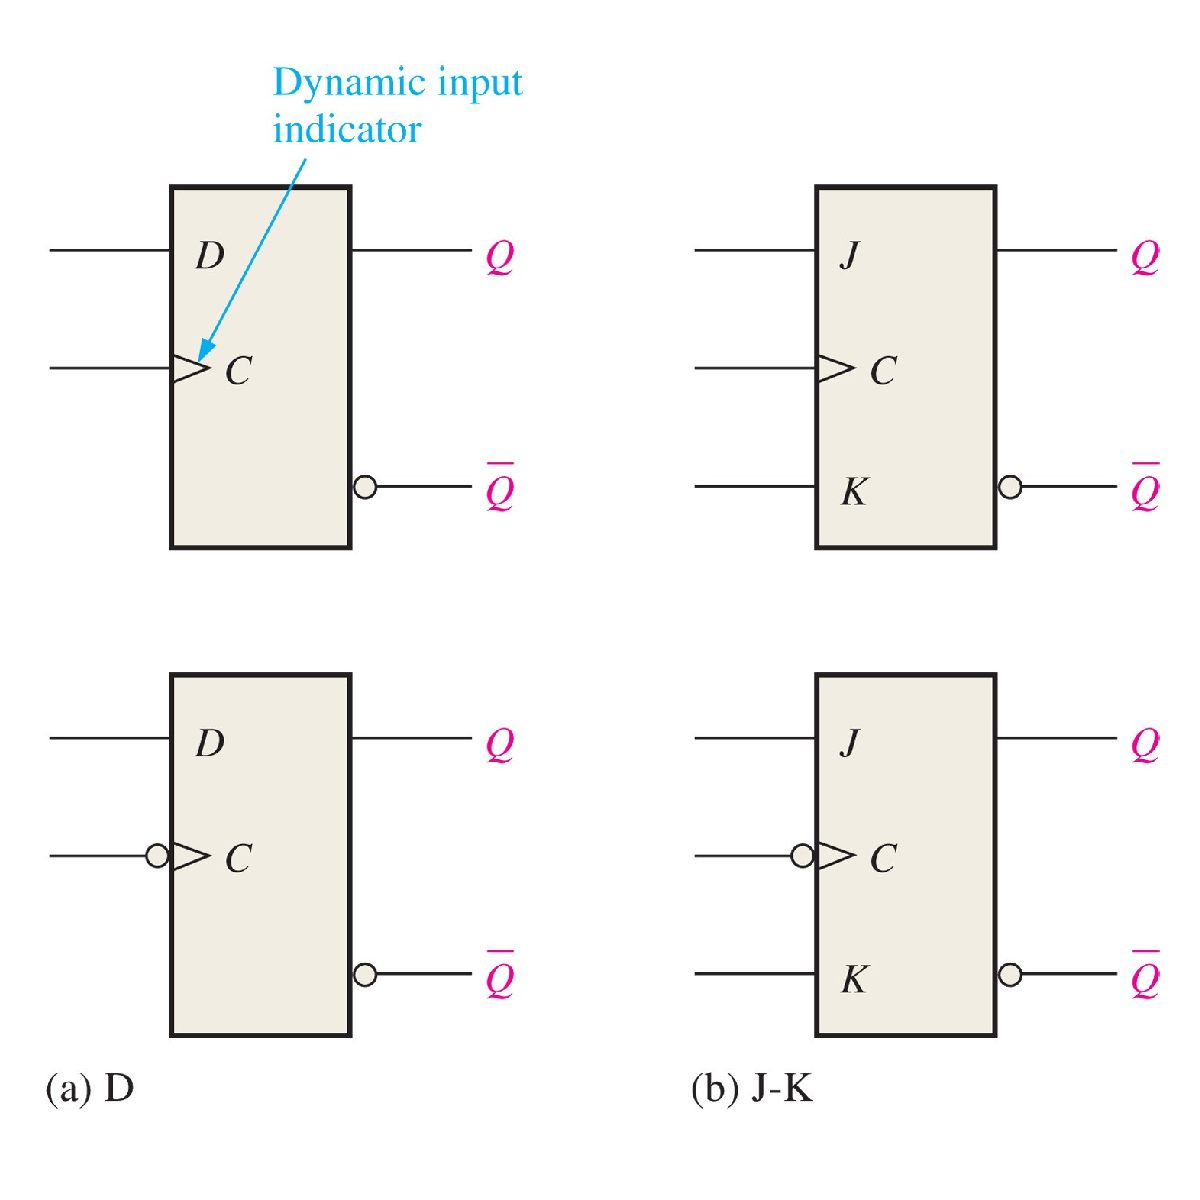
\includegraphics[width=0.6\textwidth]{figures/edge1.pdf}
\caption{\label{fig:ff1} Four types of \textbf{synchronous} latches called flip-flops.}
\end{figure}
\end{frame}

\begin{frame}{Flip-Flops}
\begin{figure}
\centering
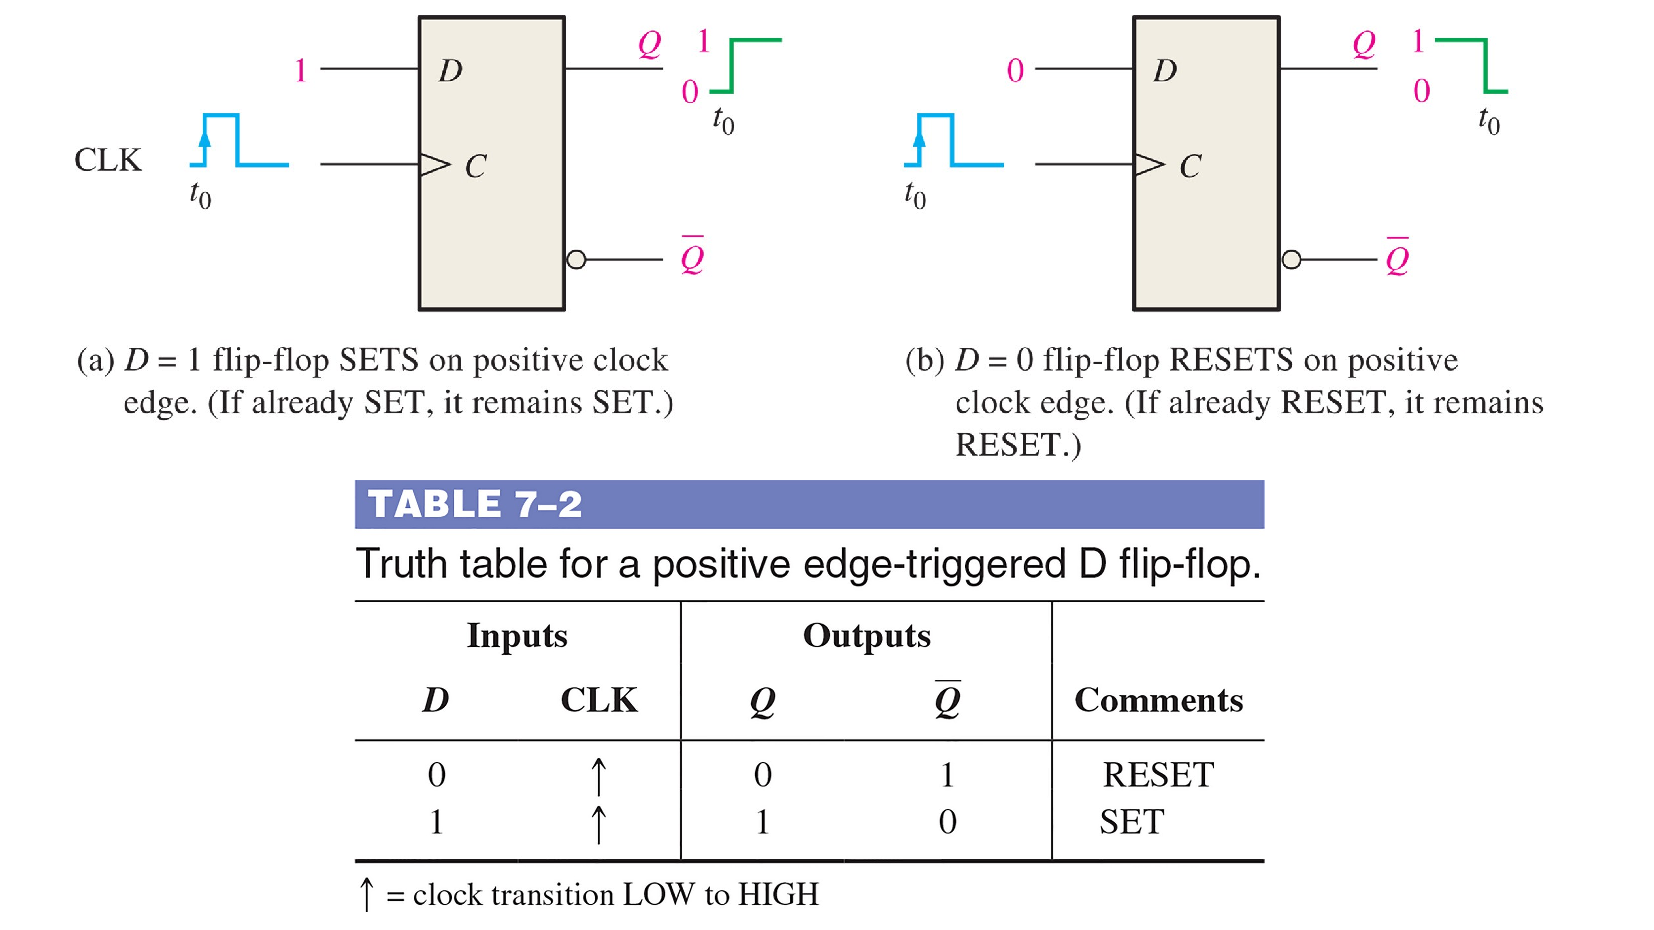
\includegraphics[width=0.75\textwidth]{figures/edge2.pdf}
\caption{\label{fig:ff2} The symbol and TT for the D-flip flop.  The behavior is simular to a D-latch without enable, but only on positive edge of clock (posedge).}
\end{figure}
\end{frame}

\begin{frame}{Flip-Flops}
\begin{figure}
\centering
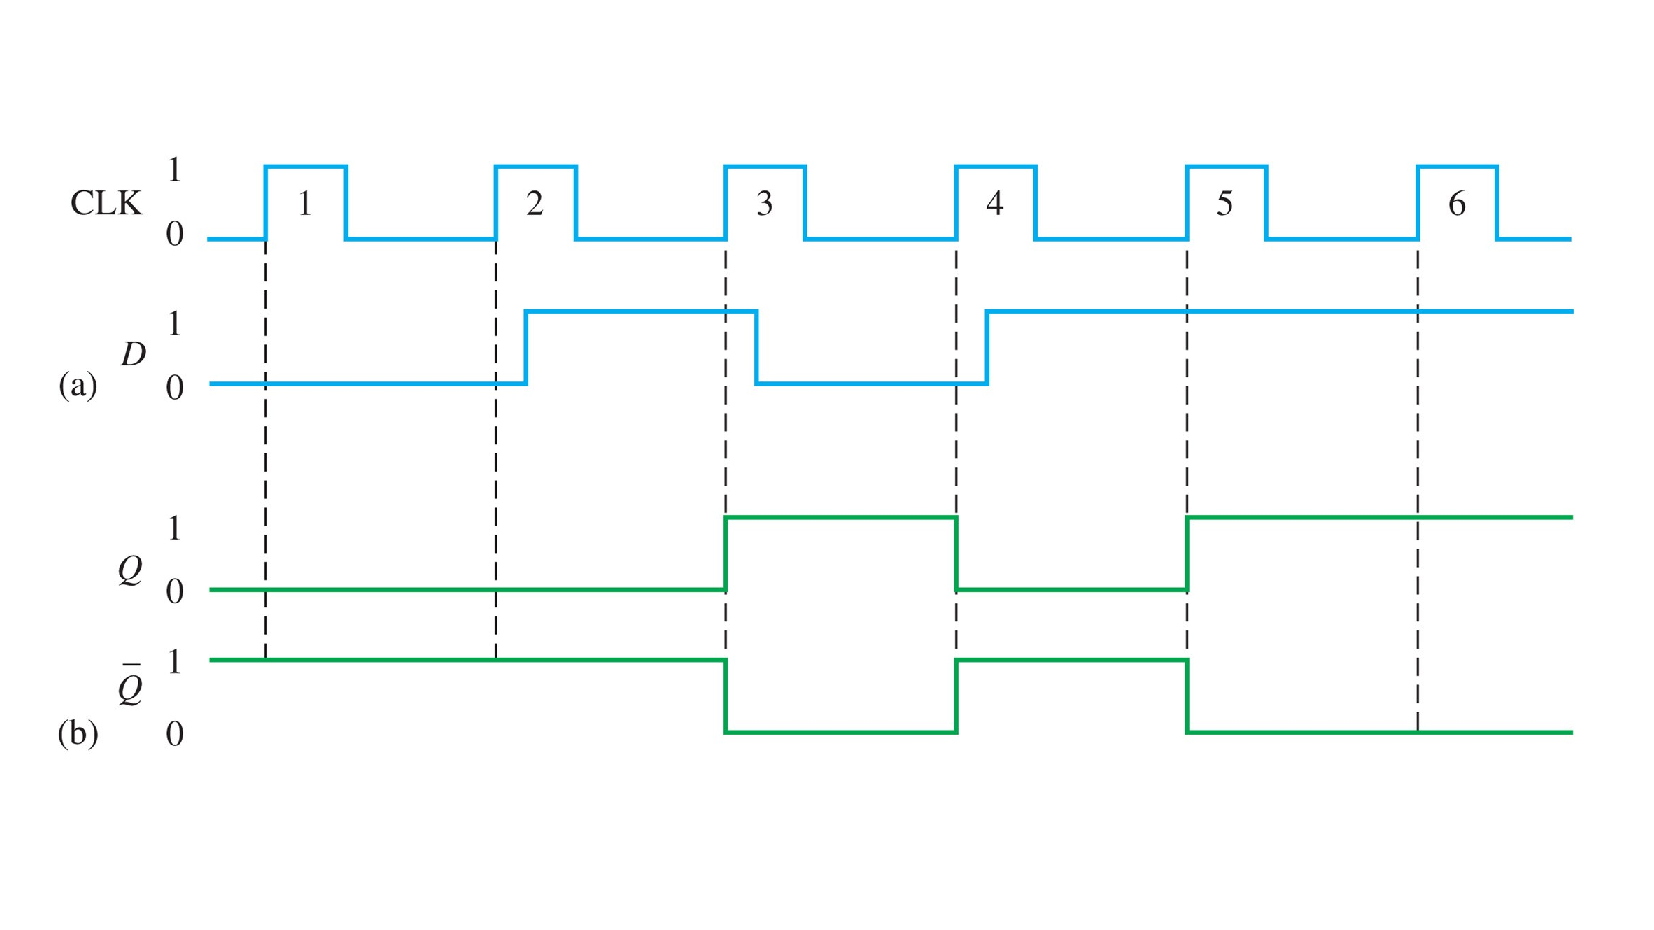
\includegraphics[width=0.75\textwidth]{figures/edge3.pdf}
\caption{\label{fig:ff3} Example of D flip-flop behavior.}
\end{figure}
\end{frame}

\begin{frame}{Flip-Flops}
\begin{figure}
\centering
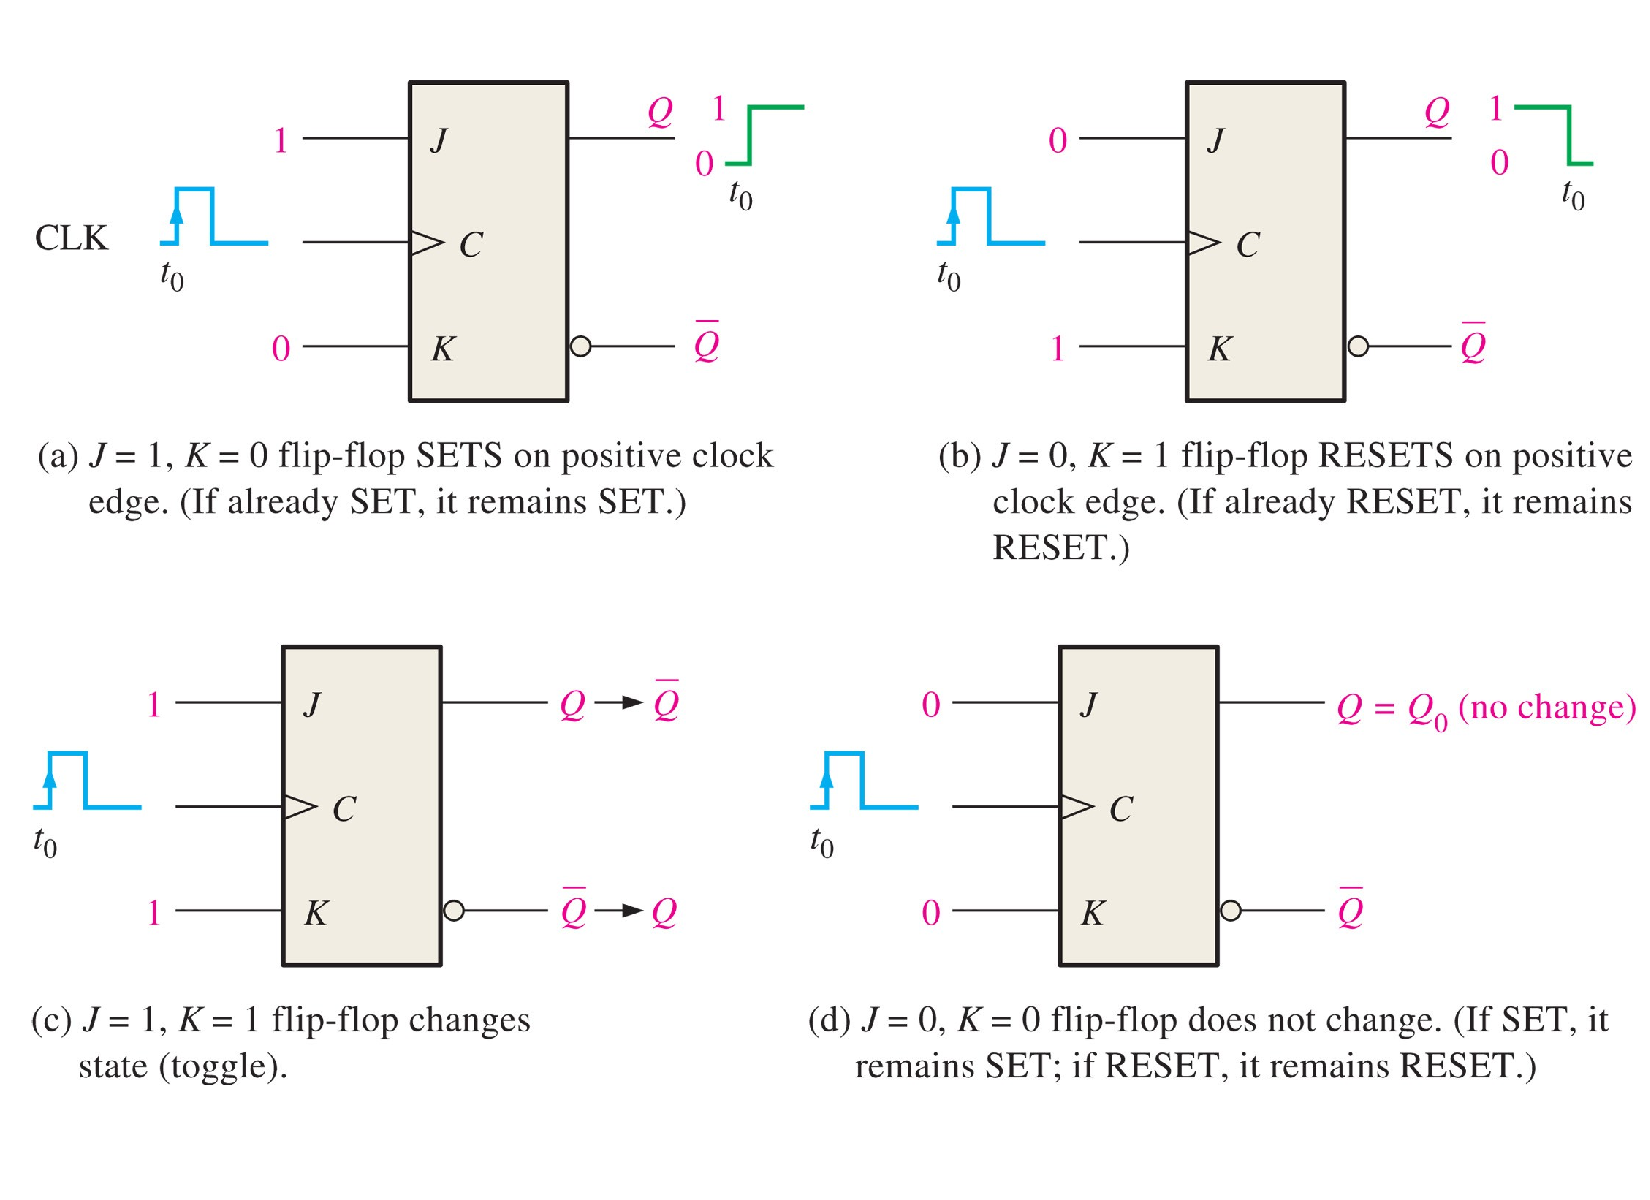
\includegraphics[width=0.75\textwidth]{figures/edge4.pdf}
\caption{\label{fig:ff4} The JK flip flop, triggered on posedge.  There are still the SET and RESET states, but the other two states differ from the SR latch.}
\end{figure}
\end{frame}

\begin{frame}{Flip-Flops}
\begin{figure}
\centering
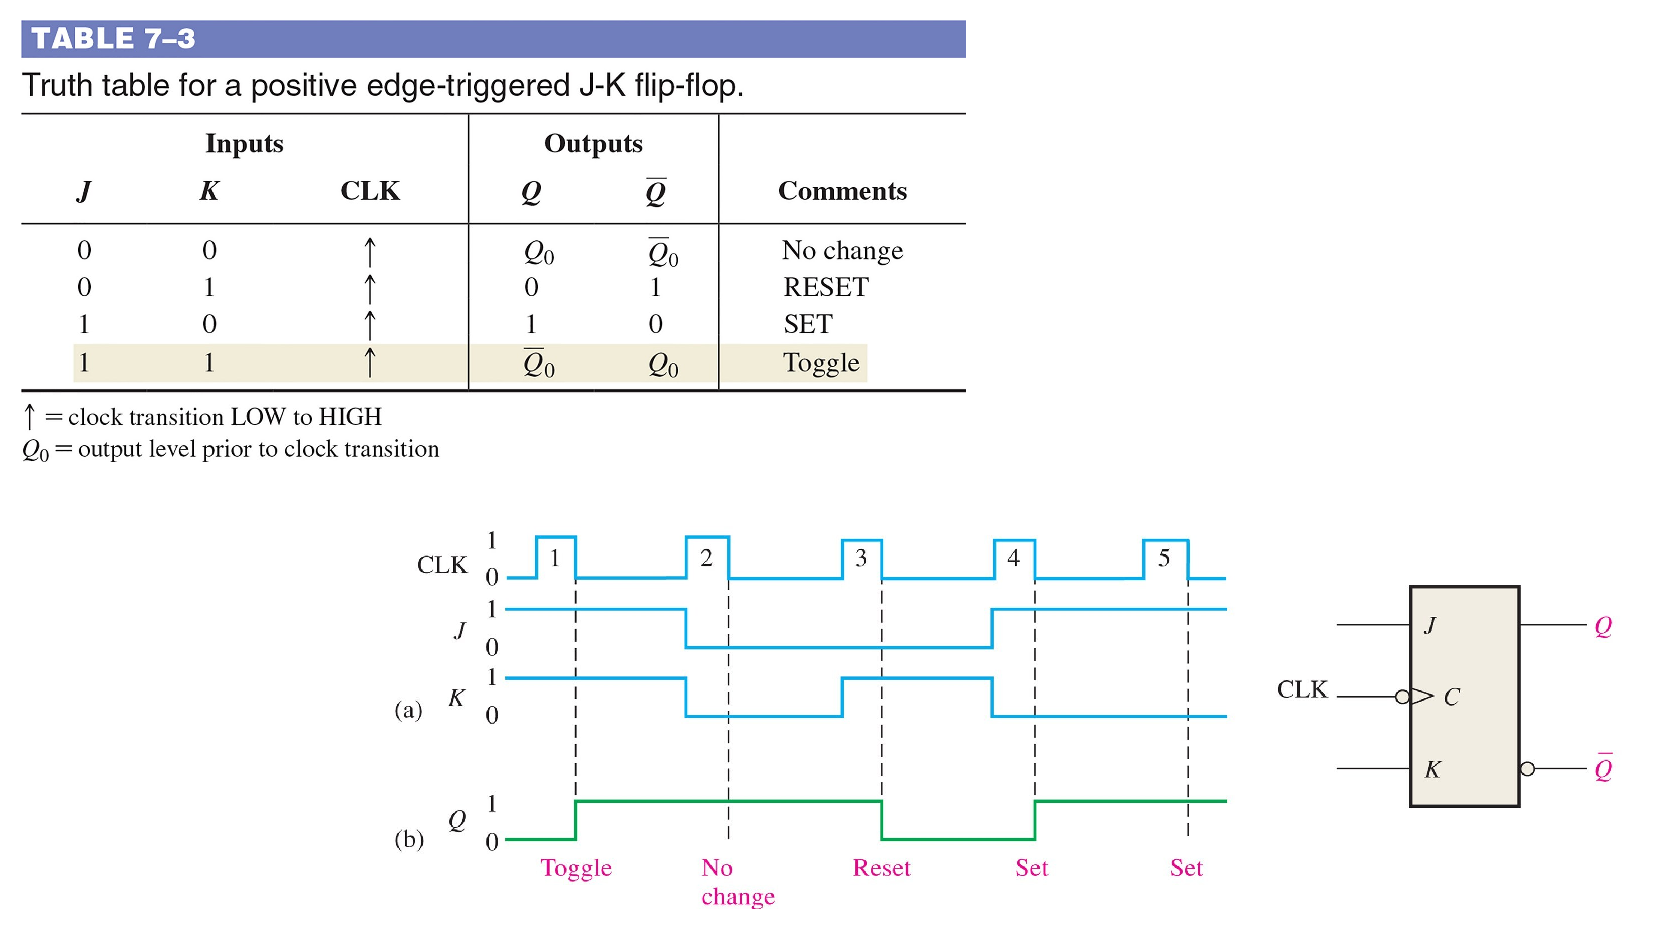
\includegraphics[width=0.75\textwidth]{figures/edge5.pdf}
\caption{\label{fig:ff5} The TT for the JK flip flop, which is also \textbf{synchronous}.  An example timing diagram is given for the JK as well.}
\end{figure}
\end{frame}

\begin{frame}{Flip-Flops}
\begin{figure}
\centering
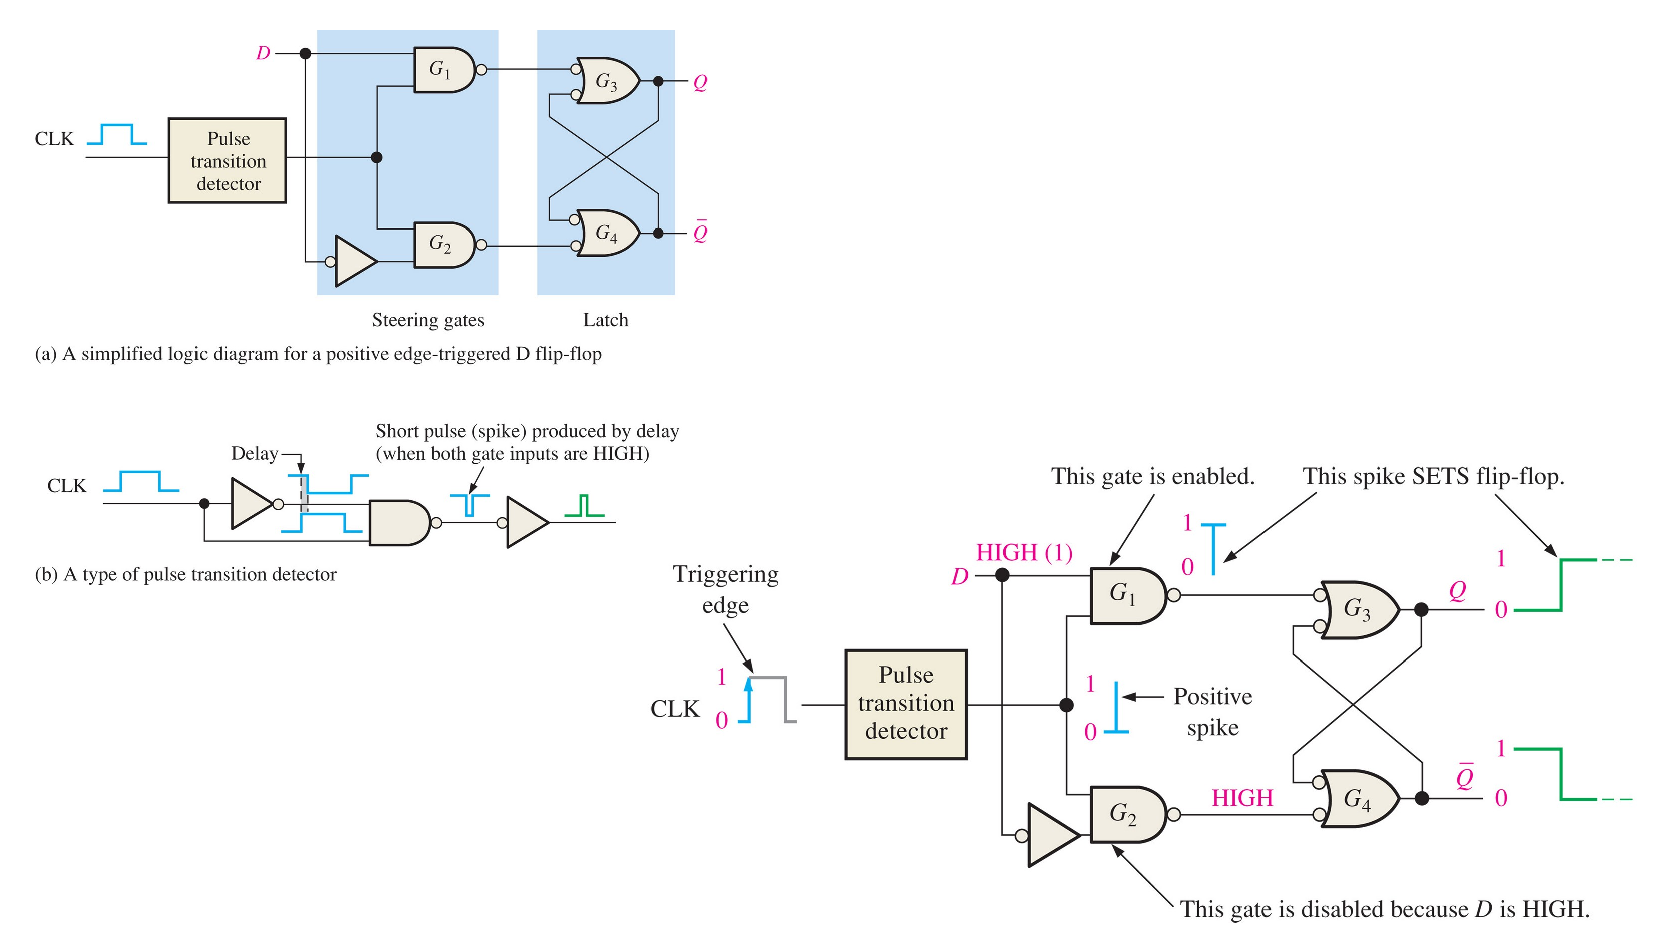
\includegraphics[width=0.75\textwidth]{figures/edge6.pdf}
\caption{\label{fig:ff6} How does the posedge triggering work?  Physically, it is based on \textit{propagation delay}.  The D flip-flop is pictured as an example, with spikes.  \textit{What counts as a spike?}}
\end{figure}
\end{frame}

\begin{frame}{Flip-Flops}
\begin{figure}
\centering
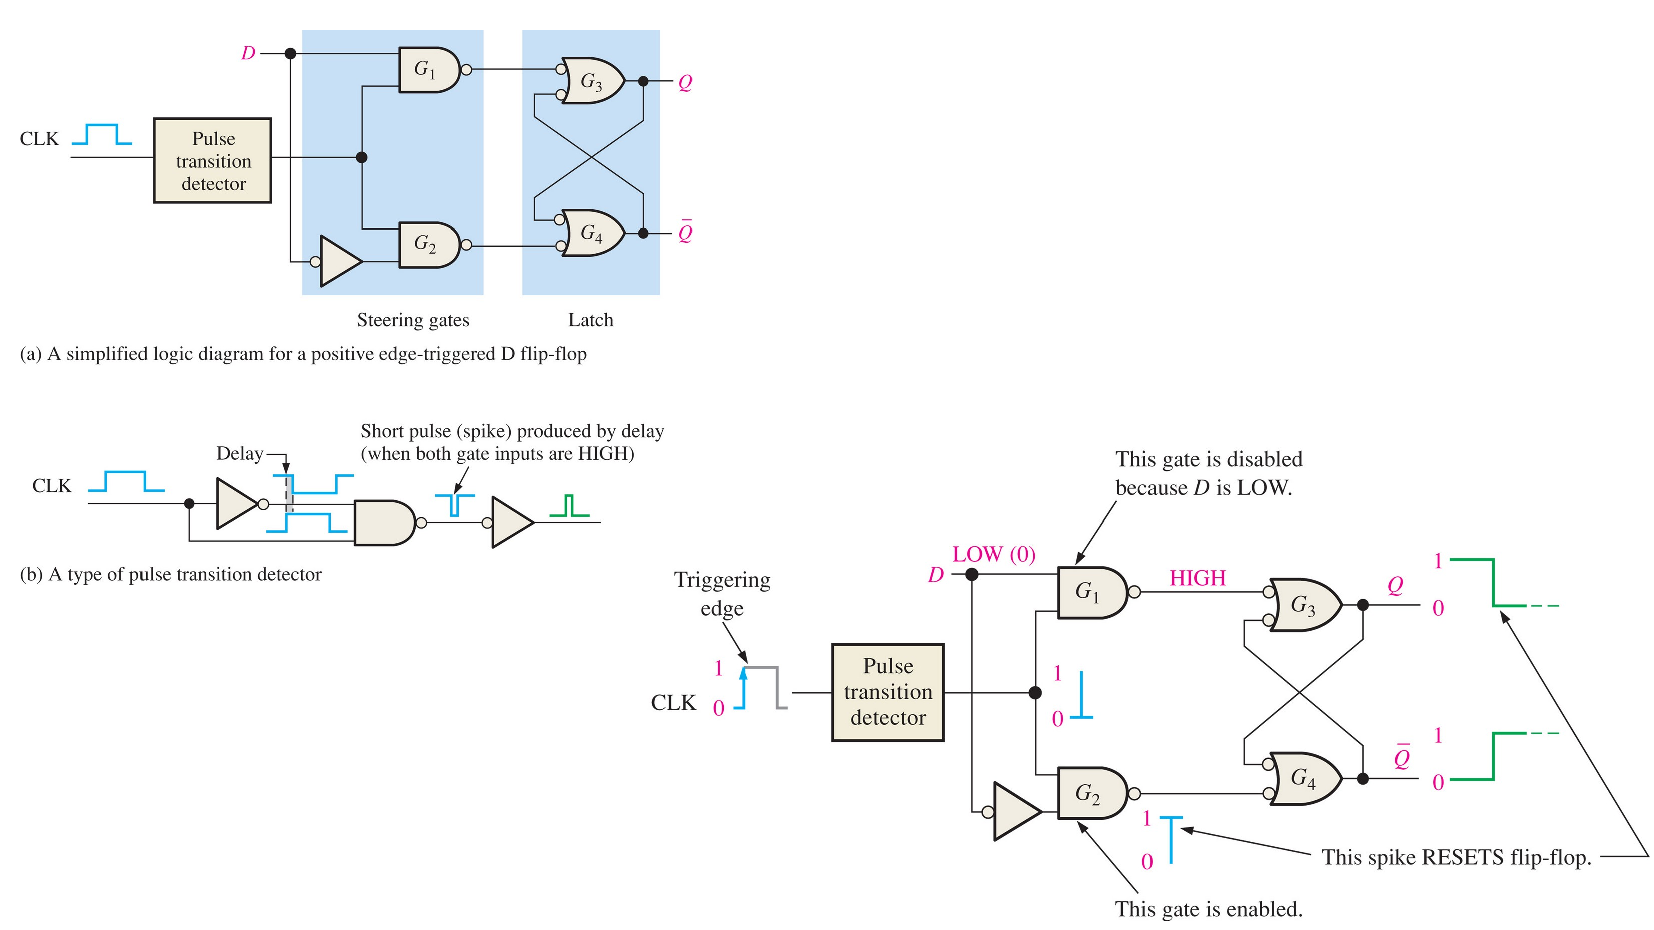
\includegraphics[width=0.75\textwidth]{figures/edge7.pdf}
\caption{\label{fig:ff7} How does the posedge triggering work?  Physically, it is based on \textit{propagation delay}.  The D flip-flop is pictured as an example, with spikes.  \textit{What counts as a spike?}}
\end{figure}
\end{frame}


\begin{frame}{Flip-Flops}
\begin{figure}
\centering
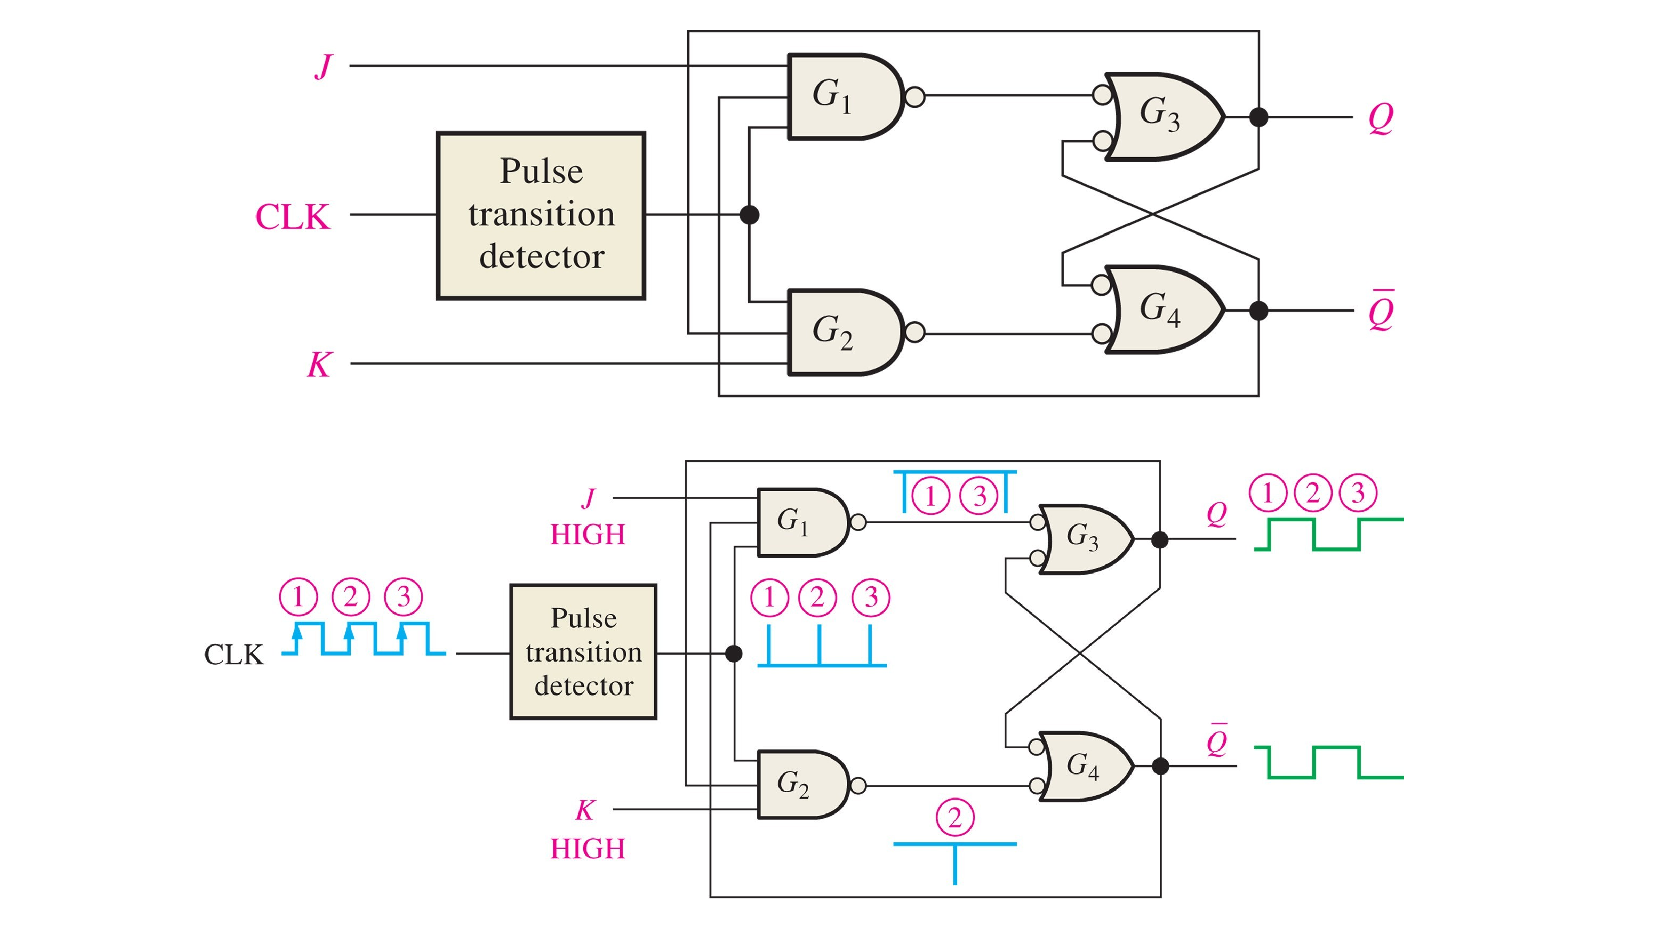
\includegraphics[width=0.75\textwidth]{figures/edge8.pdf}
\caption{\label{fig:ff8} Circuit diagram with symbols for the JK flip flop, with posedge trigger.  The JK flip-flop is in \alert{toggle} mode.}
\end{figure}
\end{frame}

\begin{frame}{Flip-Flops}
\begin{figure}
\centering
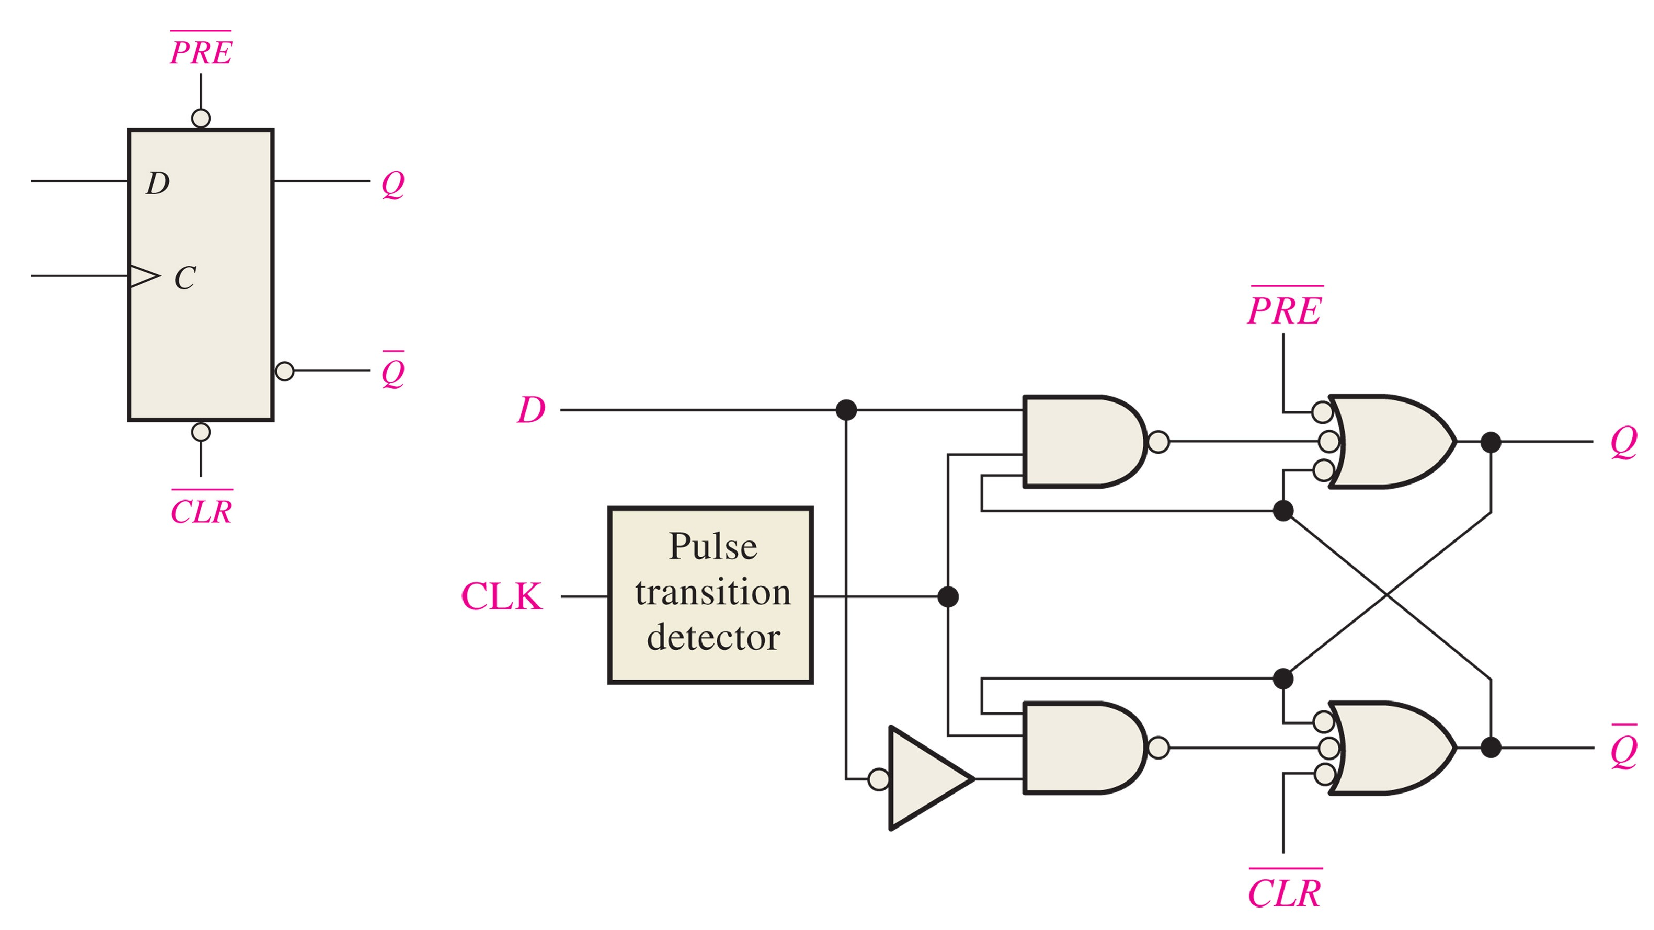
\includegraphics[width=0.75\textwidth]{figures/edge9.pdf}
\caption{\label{fig:ff9} Addig two asynchronous features, preset and clear.  These override the synchronous features due to the way they are used.}
\end{figure}
\end{frame}

\begin{frame}{Flip-Flops}
\begin{figure}
\centering
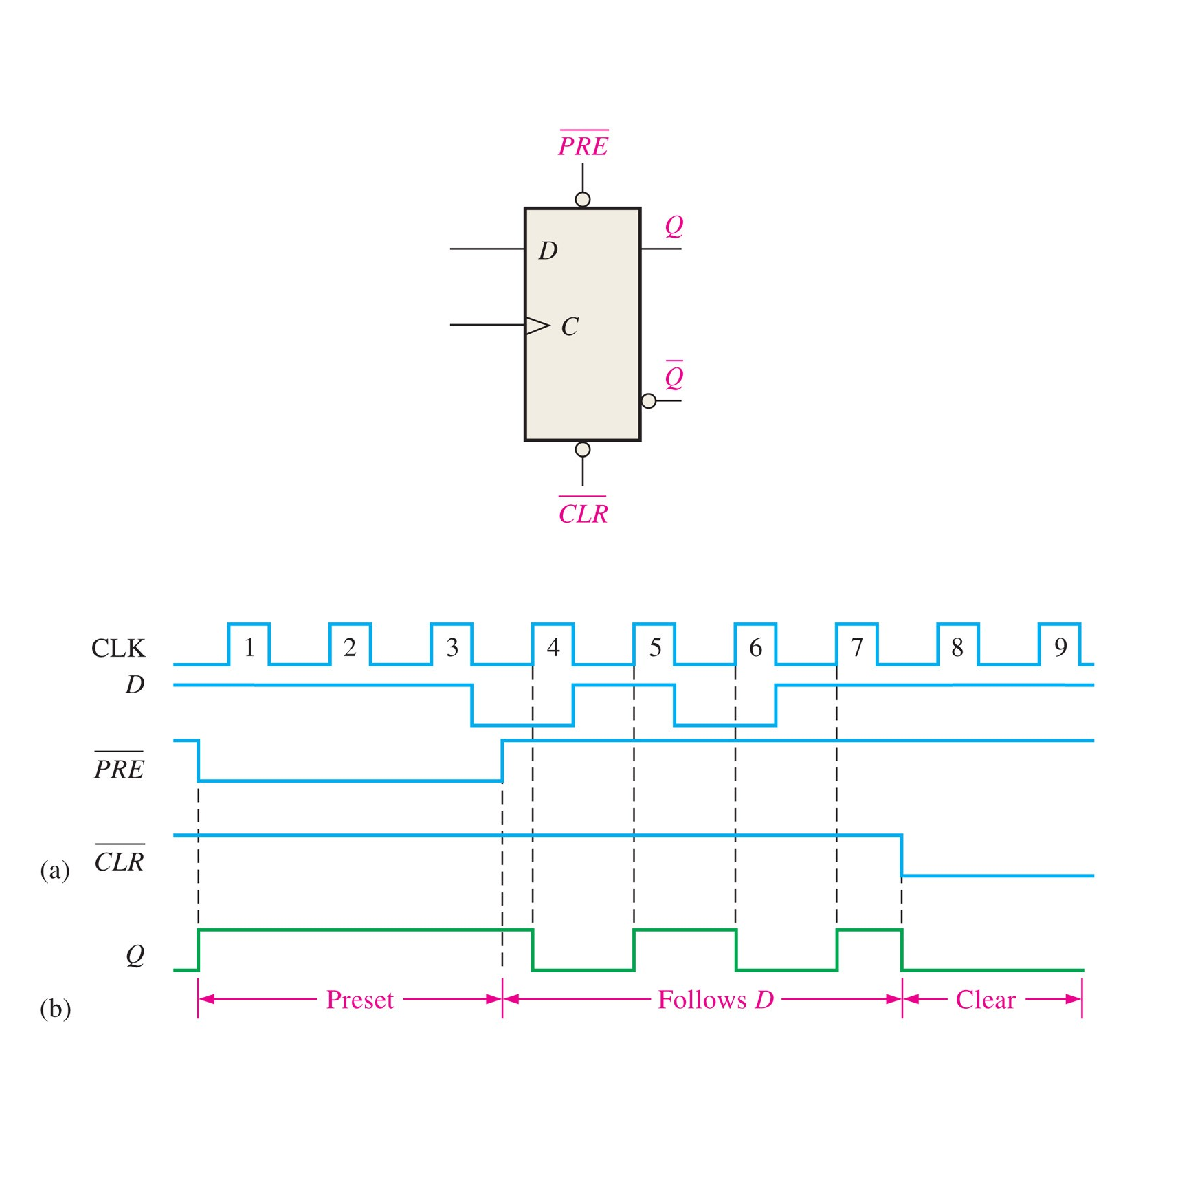
\includegraphics[width=0.75\textwidth]{figures/edge10.pdf}
\caption{\label{fig:ff10} A an example timing diagram for a JK flip-flop with active LOW present and clear.}
\end{figure}
\end{frame}

\section{Conclusion}

\begin{frame}{Unit 3 Summary}
\alert{Reading: chapter 7} \\
We now know how to generate and process digital data. We can do algebra, compare numbers, encode, decode, and multiplex.  \textit{How does memory work?  How is information held in digital systems?}
\begin{enumerate}
\item S-R latches
\begin{itemize}
\item Basic latch, de-bounce
\item Gated latch
\item D-latch
\end{itemize}
\item Flip-flops
\begin{itemize}
\item JK flip-flops
\item Synchronous vs. level-sensitive
\end{itemize}
\end{enumerate}
\end{frame}

\end{document}
